
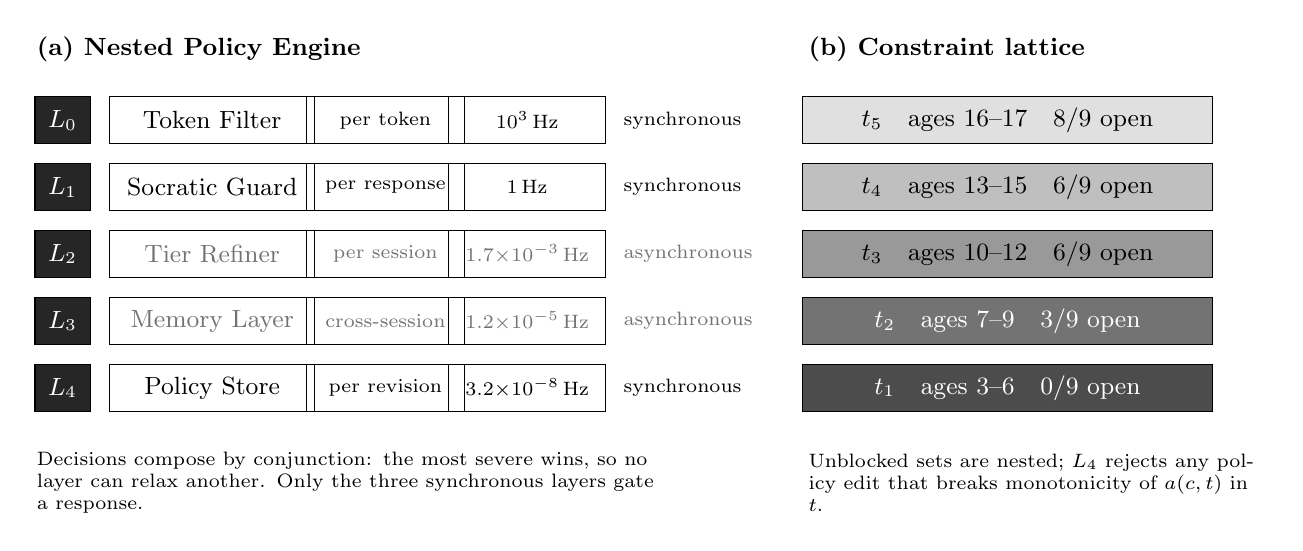
\begin{tikzpicture}[
  lbl/.style={draw, thin, rectangle, minimum width=7mm, minimum height=6mm,
              fill=black!85, text=white, font=\small},
  lname/.style={draw, thin, rectangle, minimum width=26mm, minimum height=6mm,
                font=\small},
  lcell/.style={draw, thin, rectangle, minimum width=20mm, minimum height=6mm,
                font=\scriptsize},
  tierbox/.style={draw, thin, rectangle, minimum width=52mm, minimum height=6mm,
                  font=\small},
]
\node[font=\small\bfseries, anchor=west] at (-0.45,0) {(a) Nested Policy Engine};
\node[font=\small\bfseries, anchor=west] at (9.35,0) {(b) Constraint lattice};
\node[lbl] at (0,-0.90) {$L_0$};
\node[lname] at (1.9,-0.90) {Token Filter};
\node[lcell] at (4.1,-0.90) {per token};
\node[lcell] at (5.9,-0.90) {$10^{3}$\,Hz};
\node[font=\scriptsize, anchor=west] at (7.0,-0.90) {synchronous};
\node[lbl] at (0,-1.75) {$L_1$};
\node[lname] at (1.9,-1.75) {Socratic Guard};
\node[lcell] at (4.1,-1.75) {per response};
\node[lcell] at (5.9,-1.75) {$1$\,Hz};
\node[font=\scriptsize, anchor=west] at (7.0,-1.75) {synchronous};
\node[lbl] at (0,-2.60) {$L_2$};
\node[lname, text=black!55] at (1.9,-2.60) {Tier Refiner};
\node[lcell, text=black!55] at (4.1,-2.60) {per session};
\node[lcell, text=black!55] at (5.9,-2.60) {$1.7{\times}10^{-3}$\,Hz};
\node[font=\scriptsize, text=black!55, anchor=west] at (7.0,-2.60) {asynchronous};
\node[lbl] at (0,-3.45) {$L_3$};
\node[lname, text=black!55] at (1.9,-3.45) {Memory Layer};
\node[lcell, text=black!55] at (4.1,-3.45) {cross-session};
\node[lcell, text=black!55] at (5.9,-3.45) {$1.2{\times}10^{-5}$\,Hz};
\node[font=\scriptsize, text=black!55, anchor=west] at (7.0,-3.45) {asynchronous};
\node[lbl] at (0,-4.30) {$L_4$};
\node[lname] at (1.9,-4.30) {Policy Store};
\node[lcell] at (4.1,-4.30) {per revision};
\node[lcell] at (5.9,-4.30) {$3.2{\times}10^{-8}$\,Hz};
\node[font=\scriptsize, anchor=west] at (7.0,-4.30) {synchronous};
\node[tierbox, fill=black!12, text=black] (t5) at (12.0,-0.90) {$t_5$\quad ages 16--17\quad 8/9 open};
\node[tierbox, fill=black!25, text=black] (t4) at (12.0,-1.75) {$t_4$\quad ages 13--15\quad 6/9 open};
\node[tierbox, fill=black!40, text=black] (t3) at (12.0,-2.60) {$t_3$\quad ages 10--12\quad 6/9 open};
\node[tierbox, fill=black!55, text=white] (t2) at (12.0,-3.45) {$t_2$\quad ages 7--9\quad 3/9 open};
\node[tierbox, fill=black!70, text=white] (t1) at (12.0,-4.30) {$t_1$\quad ages 3--6\quad 0/9 open};
\node[font=\scriptsize, anchor=west, text width=80mm] at (-0.45,-5.5)
  {Decisions compose by conjunction: the most severe wins, so no layer can relax
   another. Only the three synchronous layers gate a response.};
\node[font=\scriptsize, anchor=west, text width=58mm] at (9.35,-5.5)
  {Unblocked sets are nested; $L_4$ rejects any policy edit that
   breaks monotonicity of $a(c,t)$ in $t$.};
\end{tikzpicture}
